\documentclass[10pt,a4paper]{article}
\usepackage[bindingoffset=0.2in,%
            left=2.5cm,right=2cm,top=2.7cm,bottom=1in,%
            footskip=.25in]{geometry}
\usepackage[utf8]{inputenc}
\usepackage[ngerman]{babel}
\usepackage{amsmath, amsfonts, amssymb}
\usepackage{scrpage2}
\usepackage{color}
\usepackage{titlesec}
\pagestyle{scrheadings}
\usepackage{ulem, contour}
\usepackage{multicol, multirow}
\usepackage{hyperref, pdfpages, tabularx, subcaption}
\usepackage{scrextend}
\usepackage{enumerate, enumitem}
\usepackage[bottom, splitrule]{footmisc}
\usepackage{csquotes}
\usepackage{minted}

\usepackage[style=numeric, backend=biber]{biblatex}
\addbibresource{bibliography.bib}

\renewcommand{\ULdepth}{1.8pt}
\contourlength{0.8pt}

\newcommand{\cul}[1]{%
  \uline{\phantom{#1}}%
  \llap{\contour{white}{#1}}%
}

\graphicspath{
    {Images/}
}

\makeatletter
\newcommand*{\rom}[1]{\expandafter\@slowromancap\romannumeral #1@}
\makeatother

\newrobustcmd*{\parentexttrack}[1]{%
  \begingroup
  \blx@blxinit
  \blx@setsfcodes
  \blx@bibopenparen#1\blx@bibcloseparen
  \endgroup}

\AtEveryCite{%
  \let\parentext=\parentexttrack%
  \let\bibopenparen=\bibopenbracket%
  \let\bibcloseparen=\bibclosebracket}

\definecolor{gray}{rgb}{0.33, 0.33, 0.33}
\definecolor{greengreen}{rgb}{0.0, 0.56, 0.0}
\definecolor{fgreen}{rgb}{0.13, 0.55, 0.13}
\definecolor{grellow}{rgb}{0.68, 1.0, 0.18}
\definecolor{orange}{rgb}{1.0, 0.49, 0.0}
\definecolor{deepblue}{rgb}{0,0,0.5}
\definecolor{deepred}{rgb}{0.6,0,0}
\definecolor{deepgreen}{rgb}{0,0.5,0}

\usepackage{pifont}

\newcommand{\cmark}{\ding{51}}%
\newcommand{\xmark}{\ding{55}}%
\newcommand{\wontfix}{\rlap{$\square$}{\large\hspace{1pt}\xmark}}


\newcommand{\vnr}{9, 10}
\newcommand{\anr}{1}

\ihead{}
\ohead{Anfängerpraktikum 2}
\chead{Versuch \vnr, Abgabe \anr : Spule \& \linebreak Kondensator im Wechselstrom- \& Resonanzkreis}
\cfoot{\pagemark}
\setheadsepline{.5pt}
\setlength\parindent{0pt}

\begin{document}

\begin{multicols}{2}
\begin{labeling}{Versuch-Nr.:}
\item[\textcolor{white}{x}Protokollant:\hspace{38pt}] \cul{Name} \wontfix
\item[\textcolor{white}{x}Zusammenarbeit\footnotemark mit:] \cul{Name} $\square$
\item[\textcolor{white}{x}Datum:\hspace{62pt}] \cul{\today}

\columnbreak

\item[Kurs: \hspace{27pt}] \cul{Anfängerpraktikum 2}
\item[Assistent: \hspace{8.7pt}] \cul{Name}
\item[Versuch-Nr.:] \underline{\vnr}
\end{labeling}
\end{multicols}

\begin{figure}[h]
\hspace{-0.5cm}\centerline{\includegraphics[width=1.1\linewidth , height=19cm]{Deckblatt_rest}}
\end{figure}

\newpage

\tableofcontents

\vspace{10pt}

\section{Aufgabenstellung}
\begin{flushleft}
Die Versuche 9 \glqq Kondensator und Spule im Wechselstromkreis\grqq und 10 \glqq Messungen an kombinierten Wechselstromwiderständen (Resonanzkreise)\grqq behandelt die experimentelle Ermittlung physikalischer Größen an Kondensator und Spule im Wechselstromkreis. Zusätzlich werden Resonanzkreise behandelt.

Im Folgenden werden diese Versuche in \textbf{drei Abschnitte} unterteilt:

\begin{itemize}
\item[\textbf{Teil \rom{1}}:] \texttt{Versuch 9 - Teil 1, Kondensator im Wechselstromkreis.}

In diesem Teil ist es Aufgabe, die Impedanz der Kondensatoren $C_1$ und $C_2$ einzeln, sowie in Parallel- und Reihenschaltung zu bestimmen. Zusätzlich sollen die Kapazitäten der Kondensatoren ermittelt werden \cite{vers9}.

\item[\textbf{Teil \rom{2}}:] \texttt{Versuch 9 - Teil 2, Spule im Wechselstromkreis.}

Dieser Teil behandelt das verhalten der Spulen $L_1$ und $L_2$ im Wechselstromkreis. Aufgabe ist es, zunächst den Widerstand der Spulen (bei Gleichstrom) zu ermitteln und anschließend die Impedanzen und Induktivitäten zu bestimmen. Zuletzt soll der Phasenunterschied zwischen \textit{Strom} und \textit{Spannung} ermittelt und interpretiert werden \cite{vers9}.

\item[\textbf{Teil \rom{3}}:] \texttt{Versuch 10 - Resonanzkreise.}

In Teil \rom{3} werden die Ergebnisse aus Teil \rom{1} und \rom{2} verknüpft und es soll ein Resonanzschwingkreis aus den Ergebnissen dieser Teile gebildet sowie graphisch ausgewertet werden \cite{vers10}.
\end{itemize}
\end{flushleft}

\subsection{Physikalischer Hintergrund}
\begin{flushleft}
\begin{itemize}
\item[\textbf{Teil \rom{1}}:] Durch die Schaltung der Kondensatoren laden und entladen diese sich immer wieder in einem periodischen Kreislauf. Dabei wird während der ersten Halbwelle des Stromes der Kondensator zunächst entladen und dann nach überschreiten des Extremas mit umgekehrtem Vorzeichen wieder aufgeladen. Der Nulldurchgang des Stromes markiert dabei den Startpunkt der Entladung und der Punkt, an dem die Ladung auf den Kondensatorplatten unnd somit auch die Spannung am Kondensator den Maximalwert erreicht. Das bedeutet, dass die Spannungskurve um $+\frac{1}{4}$ einer Schwingunsdauer zur Stromkurve versetzt ist - dies ist eine Phasenverschiebung von $\varphi = \frac{\pi}{2}$ (Abbildung \ref{fig:zeiger_kond}) \cite{vers9}.

\begin{figure}[H]
\centering
\includegraphics[scale=0.4]{Zeiger_kond}
\caption{Zeigerdiagramm von \textcolor{blue}{Strom} und \textcolor{red}{Spannung} am Kondensator.}
\label{fig:zeiger_kond}
\end{figure}

Der fließende Wechselstrom im Kreis bei gegebener Spannung ist höher, je höher die Kapazität und die Frequenz sind, denn umso kürzer dauert der Ladungstransport zwischen den Kondensatorplatten. Es ergibt sich somit für den Wechselstromwiderstand:
\begin{equation}\label{eq:kond}
\frac{U_{eff}}{I_{eff}} = Z_C = \frac{1}{\omega \cdot C}
\end{equation}
In diesem Versuch wollen wir zudem die Parallel- und Reihenschaltung von Kondensatoren untersuchen. Dabei gilt für die Parallelschaltung der Zusammenhang
\begin{equation}\label{eq:kond_para}
C_{ges} = \sum_i C_i
\end{equation}
Für die Reihenschaltung gilt der Zusammenhang über die Kehrwerte:
\begin{equation}\label{eq:kond_reihe}
\frac{1}{C_{ges}} = \sum_i \frac{1}{C_i}
\end{equation}

\item[\textbf{Teil \rom{2}}:] Bei der Spule im Wechselstromkreis verhält es sich ähnlich zum Kondensator. Wir müssen hierbei jedoch zunächst zwischen einer \textit{idealen} Spule und einer Spule in der Realität unterscheiden. Erste bezeichnet dabei eine Spule \textit{ohne} ohmschen Drahtwiderstand - dies ist in unserem Versuch nicht gegeben. Deshalb wollen wir zunächst den Drahtwiderstand bestimmen, der ganz einfach nach dem Ohmschen Gesetz bei \textbf{Gleichspannung} zu ermitteln ist:
\begin{equation}\label{eq:spule_gleichspannung}
I_{=} = \frac{U_{=}}{R}
\end{equation}
Beim anlegen einer Wechselspannung an die Spule fließt dann ein Wechselstrom, der mit einem sich in gleichem Rhythmus ändernden Magnetfeld verbunden ist. Dieses Magnetfeld nimmt während der ersten Halbwelle des Stromes zu und mit abnehmendem Strom ebenfalls wieder ab. Nach dem \textbf{Induktionsgesetz} ist ist ein sich zeitlich änderndes Magnetfeld mit einer induzierten Spannung $U_{ind}$ verknüpft. Hierbei wird das Magnetfeld durch den Strom der Spule erzeugt, weshalb beim Nulldurchgang des Stromes die Spannung an der Spule maximal ist (und im Maximum des Stromes ist sie Null). Somit besteht eine umgekehrte Phasenverschiebung zum Kondensator; die Stromkurve ist hier um $- \frac{1}{4}$ zur Stromkurve versetzt - eine Phasenverschiebung von $\varphi = - \frac{pi}{2}$ (Abbildung \ref{fig:zeiger_spule}) \cite{vers9}.

\begin{figure}[H]
\centering
\includegraphics[scale=0.4]{Zeiger_spule}
\caption{Zeigerdiagramm von \textcolor{blue}{Strom} und \textcolor{red}{Spannung} an der Spule.}
\label{fig:zeiger_spule}
\end{figure}

Der Wechselstrom, der durch die Spule fließt ist hier umso kleiner, je höher die Frequenz und je höher die Selbstinduktion (Induktivität $L$), da die Geschwindigkeit der Stromänderung und die Größe der Induktivität die Ausbildung des Stromes bremsen. Für die \textit{ideale} Spule gilt hier der Zusammenhang der Größen ähnlich zum Kondensator:
\begin{equation}\label{eq:spule_id}
\frac{U_{eff}}{I_{eff}} = Z_L = \omega \cdot L
\end{equation}

In unserem Experiment besitzen wir jedoch \textbf{keine} ideale Spule und müssen somit zusätzlich den Drahtwiderstand beachten. Dafür betrachtet man Spule und Drahtwiderstand als Reihenschaltung. Es ergibt sich:
\begin{equation}\label{eq:spule}
\frac{U_{eff}}{I_{eff}} = Z_{R+L} = \sqrt{R^{2} + \omega^2 \cdot L^2}
\end{equation}

Die Induktivität $L$ einer Spule kann durch die Verwendung ferromagnetischer Stoffe verändert - vergrößert - werden. Dabei sind die Qualität und Einschubtiefe des Materials maßgeblich für die Auswirkungen.

\item[\textbf{Teil \rom{3}}:] \hypertarget{theo-res}{Werden} eine Spule und ein Kondensator in einen Wechselstromkreis geschalten, bilden sie einen \textbf{elektromagnetischen Schwingkreis}, wie Abbildung \ref{fig:schemschwing} schematisch zeigt. Dabei wollen wir Reihen- und Parallelschwingkreise betrachten \cite{vers10}.

\begin{figure}[H]
\centering
\includegraphics[scale=0.4]{schema_schwing}
\caption{Schematischer Schaltplan eines Reihenschwingkreises \cite{vers10}.}
\label{fig:schemschwing}
\end{figure}

Wird ein Schwingkreis einmal angestoßen, führt er Schwingungen mit einer Eigenfrequenz $f_E$ aus. Mit der Zeit wird diese Schwingung jedoch durch Dämpfungsverluste, wie ohmsche Widerstände und die Emission elektromagnetischer Wellen, gebremst. Um dieser Dämpfung entgegen zu wirken kann man den Schwingkreis von außen periodisch anregen (Anregefrequenz $f_A$). Im Falle, dass die Anregerfrequenz der Eigenfrequenz des Schwingkreises entspricht ($f_A = f_E$), spricht man von \textbf{Resonanz} - großen Peaks der Amplituden von Strom und Spannung. Dabei heben sich die Beträge der Induktivität und der Kapazität zum Gesamtwiderstand auf:
\begin{equation}\label{eq:reso}
\omega L - \frac{1}{\omega C} = 0
\end{equation}
Die Resonanzfrequenz ist dadurch gegeben mit
\begin{equation}\label{eq:res_freq}
\omega_{res} = \frac{1}{\sqrt{LC}}
\end{equation}
Diese Formel ist auch als \texttt{THOMSON}-Formel bekannt. Diese Formel können wir zur Berechnung der benötigten Kapazität in unserem Schwingkreis umstellen:
\begin{align}\label{eq:berechn_kapa}
\omega L = \frac{1}{\omega C} \hspace{10pt}\Rightarrow \hspace{10pt} C = \frac{1}{\omega^2 L}
\end{align}

Bei einer völlig Dämpfungsfreien Schwingung kann die Resonanz die Zerstörung des Systems bewirken (\textit{Resonanzkatastrophe}).
\end{itemize}
\end{flushleft}

\newpage

\section{Messmethoden}
\begin{flushleft}
Wir führen diesen Versuch als \textbf{Simulationsversuch} mit der Software \texttt{LTSpice} durch\footnote{Mehr Infos und Download: \href{https://www.analog.com/en/design-center/design-tools-and-calculators/ltspice-simulator.html}{LTSpice website}}.
\end{flushleft}

\subsection{Versuchsaufbau}
\begin{flushleft}
Da wir wie bereits angesprochen eine Simulation durchführen benötigen wir nur einen Computer mit der Software \texttt{LTSpice}. Zusätzlich haben wir für diesen Versuch einen Ordner mit den Objekten, die verwendet werden sollen, erhalten. Grundsätzlich können jedoch beliebige Kondensatoren und Spulen verwendet werden; es müssen dann nur u.U. Anpassungen vorgenommen werden.
\end{flushleft}

\subsection{Schaltpläne}
\begin{flushleft}
Die folgenden Schaltbilder sind screenshots aus dem Simulationsprogramm.

% KONDENSATOREN:
\begin{figure}[H]
\centering
\begin{subfigure}{0.5\linewidth}
\centering
\includegraphics[scale=0.5]{Schalt_V9_Kond1}
\subcaption{Kondensator $C_1$.}
\label{fig:schalt_v9_kond1}
\end{subfigure}%
%
\begin{subfigure}{0.5\linewidth}
\centering
\includegraphics[scale=0.5]{Schalt_V9_Kond2}
\subcaption{Kondensator $C_2$.}
\label{fig:schalt_v9_kond2}
\end{subfigure}%

\begin{subfigure}{0.5\linewidth}
\centering
\includegraphics[scale=0.5]{Schalt_V9_para}
\subcaption{Kondensator Parallelschaltung $C_{\parallel}$.}
\label{fig:schalt_v9_para}
\end{subfigure}%
%
\begin{subfigure}{0.5\linewidth}
\centering
\includegraphics[scale=0.5]{Schalt_V9_reihe}
\subcaption{Kondensator Reihenschaltung $C_{\mid}$.}
\label{fig:schalt_v9_reihe}
\end{subfigure}%
\caption{Schaltungen zu Teil \rom{1} - Kondensator im Wechselstromkreis.}
\label{fig:SCHALT_KOND}
\end{figure}

% SPULEN:
\begin{figure}[H]
\begin{subfigure}{0.5\linewidth}
\centering
\includegraphics[scale=0.4]{Schalt_V9_Spule1}
\subcaption{Schaltung Teil \rom{2}: Spule $L_1$.}
\label{fig:schalt_v9_t2_spule1}
\end{subfigure}%
% --
\begin{subfigure}{0.5\linewidth}
\centering
\includegraphics[scale=0.4]{Schalt_V9_Spule2}
\subcaption{Schaltung Teil \rom{2}: Spule $L_2$.}
\label{fig:schalt_v9_t2_spule2}
\end{subfigure}%
\caption{Schaltungen zu Teil \rom{2} - Spulen im Wechselstromkreis.}
\label{fig:SCHALT_SPULE}
\end{figure}

\newpage
\begin{figure}[H]
\centering
\begin{subfigure}{0.5\linewidth}
\centering
\includegraphics[scale=0.4]{V10_Konds}
\subcaption{\centering Aufbau der Kondensatoren für den Resonanzschwingkreis.}
\label{fig:schalt_v10_konds}
\end{subfigure}%

\begin{subfigure}{0.5\linewidth}
\centering
\includegraphics[scale=0.4]{Schalt_v10_reihe}
\subcaption{Aufbau des Reihenschwingkreises.}
\label{fig:schalt_v10_schwi_reihe}
\end{subfigure}%
% --
\begin{subfigure}{0.5\linewidth}
\centering
\includegraphics[scale=0.4]{Schalt_v10_para}
\subcaption{Aufbau des Parallelschwingkreises.}
\label{fig:schalt_v10_schwi_para}
\end{subfigure}%

\caption{Schaltungen zu Teil \rom{3} - Resonanzkreise}
\label{fig:SCHALT_RESO}
\end{figure}
Auf die genaue Bedeutung und Herkunft von Abbildung \ref{fig:schalt_v10_konds} wird im Abschnitt zu den \hyperlink{sec:erg_resk}{Versuchsergebnissen zum Resonanzkreis} genauer eingegangen.
\end{flushleft}

\section{Versuchsdurchführung}
\begin{flushleft}
Wir bauen die Schaltbilder der Abbildungen \ref{fig:SCHALT_KOND}, \ref{fig:SCHALT_SPULE} und \ref{fig:SCHALT_RESO} nacheinander auf.

Wir messen für die Kondensatoren die \textbf{Effektivstromstärke} $I_{eff}$ und berechnen mit dieser und der \textbf{Effektivspannung} $U_{eff}$ dann die Impedanz und die Kapazität der Kondensatoren in Einzel-, Parallel- und Reihenschaltung.

Für die Spulen gehen wir ähnlich vor. Auch hier wollen wir die Effektivwerte bestimmen und mit diesen die Impedanz und die Induktivität berechnen. Das Vorgehen ist analog zu dem mit den Kondensatoren, nur dass wir hier die Einschubtiefe der Kerne variieren und nur jeweils eine Einzelschaltung der beiden Spulen betrachten.
\end{flushleft}
\begin{flushleft}
Zuletzt wollen wir aus den Komponenten noch einen elektromagnetischen Schwingkreis aufbauen. Dazu bauen wir die entsprechenden SChaltungen auf und werten den Schwingkreis garphisch aus (wieder die Effektivwerte) (Siehe auch: \hyperlink{sec:erg_resk}{Versuchsergebnisse - Resonanzkreis}).
\end{flushleft}

\paragraph{Bestimmung der Effektivstromstärke $I_{eff}$}
\begin{flushleft}
Wir bestimmen die \textbf{Effektivstromstärke} $I_{eff}$ mit Hilfe des Simulationsprogrammes durch den Befehl \texttt{.meas \textit{name} rms(\textit{Quelle}}). Dadurch wird die \textit{Root-Mean-Square} über die Stromstärke am Punkt \textit{Quelle} (der Punkt sollte direkt an der Komponente liegen) gebildet und in der \texttt{.log}-Datei gespeichert. Diese kann dann ausgelesen und zur weiteren Verarbeitung genutzt werden (Mein verwendetes script ist im \hyperlink{sec:appendix}{Appendix} beigelegt).
\end{flushleft}

\newpage

\section{Versuchsergebnisse}
\begin{flushleft}
\hypertarget{VersErg}{}
\begin{itemize}
\item[\textbf{Teil \rom{1}}:] \texttt{Kondensator im Wechselstromkreis}

Für die Berechnungen mit den Kondensatoren bestimmen wir zunächst die \textbf{Effektivspannung} $U_{eff}$, die durch $U_{eff} = \frac{\hat{U}}{\sqrt{2}}$ gegeben ist, wobei $\hat{U}$ die Amplitude der Spannung beschreibt. In unserem Fall beträgt die Amplitude $10 V$.

\begin{table}[h]
\centering
\caption{Messergebnisse and den Kondensatorschaltungen.\protect\footnotemark}
\label{tab_messerg_kond}
\begin{tabular}{|c|c|c|c|c|c|c|c|c|c|c|}
\hline
& $U_{eff} (V)$ & $I_{eff} (A)$ & $\omega (Hz)$ & $Z (\Omega)$ & $C (F)$ \\
\hline
$C_1$ & 7.071 & 0.227349 & 314 & 31.102 & $102.395 \cdot 10^{-6}$ \\ 
\hline 
$C_2$ & 7.071 & 0.0339359 & 314 & 208.365 & $15.284 \cdot 10^{-6}$ \\ 
\hline 
$C_{\parallel}$ & 7.071 & 0.261285 & 314 & 27.063 & $117.679 \cdot 10^{-6}$ \\ 
\hline 
$C_{\mid}$ & 7.071 & 0.0295282 & 314 & 239.468 & $13.299 \cdot 10^{-6}$ \\ 
\hline 
\end{tabular}
\normalsize
\end{table}
\footnotetext{Die Ergebnisse sind ohne absolute Fehler angegeben, da aus der Simulation mit \textit{LTSpice} keine entnommen werden können.}

Aus den Messwerten für die Effektivwerte haben wir nun die Impedanzen sowie die Kapazitäten bestimmt. Wir greifen später in \textbf{Teil \rom{3}} auf diese zurück.

\item[\textbf{Teil \rom{2}}:] \texttt{Spule bei Gleichstrom und im Wechselstromkreis}

Ergebnisse der Spulen bei Gleichstrom: $I_{Massiv} = 0.4A$, $I_{Lamell} = 0.384A$.

Die Drahtwiderstände betragen somit (ohne Kern\footnote{Die Spulen sind lediglich nach ihren Kernen benannt.}):
\begin{align*}
R_{Massiv} &= \frac{U}{I_{Massiv}} = \frac{5 V}{0.4 A} = 12.5 \Omega & R_{Lamell} &= \frac{U}{I_{Lamell}} = \frac{5 V}{0.384 A} \approx 13.02 \Omega
\end{align*}

Mit diesen Werten für den Drahtwiderstand an der jeweiligen Spule können wir die Impdeanz und Induktivität der Spulen mit Gleichung \ref{eq:spule} berechnen.

\begin{table}[H]
\centering
\centerline{
\begin{subtable}[t]{.6\textwidth}
\centering
\subcaption{Messergebnisse an der Spule 1 (Massivkern).}
\normalsize
\tiny
\begin{tabular}{|c|c|c|c|c|c|}
\hline
$x (cm)$ & $I_{eff} (A)$ & $U_{eff} (V)$ & $\omega (Hz)$ & $Z (\Omega)$ & $L (H)$ \\
\hline
0 & 0.233 & 7.072 & 314 & 30.43 & 0.089 \\ 
\hline
0.5 & 0.226 & 7.072 & 314 & 31.373 & 0.092 \\ 
\hline
1 & 0.219 & 7.072 & 314 & 32.325 & 0.095 \\ 
\hline
1.5 & 0.213 & 7.072 & 314 & 33.317 & 0.099 \\ 
\hline
2 & 0.206 & 7.072 & 314 & 34.376 & 0.102 \\ 
\hline
2.5 & 0.2 & 7.072 & 314 & 35.53 & 0.106 \\ 
\hline
3 & 0.193 & 7.072 & 314 & 36.806 & 0.111 \\ 
\hline
3.5 & 0.185 & 7.072 & 314 & 38.227 & 0.116 \\ 
\hline
4 & 0.178 & 7.072 & 314 & 39.82 & 0.121 \\ 
\hline
4.5 & 0.17 & 7.072 & 314 & 41.605 & 0.127 \\ 
\hline
5 & 0.163 & 7.072 & 314 & 43.604 & 0.134 \\ 
\hline
5.5 & 0.155 & 7.072 & 314 & 45.835 & 0.141 \\ 
\hline
6 & 0.147 & 7.072 & 314 & 48.317 & 0.149 \\ 
\hline
6.5 & 0.139 & 7.072 & 314 & 51.063 & 0.158 \\ 
\hline
7 & 0.131 & 7.072 & 314 & 54.085 & 0.168 \\ 
\hline
7.5 & 0.124 & 7.072 & 314 & 57.396 & 0.179 \\ 
\hline
8 & 0.116 & 7.072 & 314 & 60.999 & 0.191 \\ 
\hline
8.5 & 0.109 & 7.072 & 314 & 64.903 & 0.203 \\ 
\hline
9 & 0.103 & 7.072 & 314 & 69.106 & 0.217 \\ 
\hline
9.5 & 0.097 & 7.072 & 314 & 73.608 & 0.232 \\ 
\hline
10 & 0.091 & 7.072 & 314 & 78.405 & 0.247 \\ 
\hline
10.5 & 0.085 & 7.072 & 314 & 83.487 & 0.263 \\ 
\hline
11 & 0.08 & 7.072 & 314 & 88.843 & 0.281 \\ 
\hline
11.5 & 0.075 & 7.072 & 314 & 94.459 & 0.299 \\ 
\hline
12 & 0.071 & 7.072 & 314 & 100.315 & 0.317 \\ 
\hline
12.5 & 0.067 & 7.072 & 314 & 106.39 & 0.337 \\ 
\hline
13 & 0.063 & 7.072 & 314 & 112.662 & 0.357 \\ 
\hline
13.5 & 0.06 & 7.072 & 314 & 119.099 & 0.378 \\ 
\hline
14 & 0.057 & 7.072 & 314 & 125.677 & 0.399 \\ 
\hline
14.5 & 0.054 & 7.072 & 314 & 132.361 & 0.42 \\ 
\hline
15 & 0.051 & 7.072 & 314 & 139.121 & 0.442 \\ 
\hline
15.5 & 0.049 & 7.072 & 314 & 145.924 & 0.464 \\ 
\hline
16 & 0.047 & 7.072 & 314 & 152.735 & 0.485 \\ 
\hline
16.5 & 0.045 & 7.072 & 314 & 159.52 & 0.507 \\ 
\hline
17 & 0.043 & 7.072 & 314 & 166.252 & 0.528 \\ 
\hline
17.5 & 0.041 & 7.072 & 314 & 172.895 & 0.55 \\ 
\hline
18 & 0.04 & 7.072 & 314 & 179.419 & 0.571 \\ 
\hline
18.5 & 0.039 & 7.072 & 314 & 185.803 & 0.591 \\ 
\hline
19 & 0.037 & 7.072 & 314 & 192.025 & 0.611 \\ 
\hline
19.5 & 0.036 & 7.072 & 314 & 198.06 & 0.63 \\ 
\hline
20 & 0.035 & 7.072 & 314 & 203.891 & 0.649 \\ 
\hline
20.5 & 0.034 & 7.072 & 314 & 209.506 & 0.667 \\ 
\hline
21 & 0.033 & 7.072 & 314 & 214.893 & 0.684 \\ 
\hline
21.5 & 0.033 & 7.072 & 314 & 220.044 & 0.7 \\ 
\hline
22 & 0.032 & 7.072 & 314 & 224.954 & 0.716 \\ 
\hline
22.5 & 0.031 & 7.072 & 314 & 229.618 & 0.731 \\ 
\hline
23 & 0.031 & 7.072 & 314 & 234.039 & 0.745 \\ 
\hline
23.5 & 0.03 & 7.072 & 314 & 238.214 & 0.758 \\ 
\hline
24 & 0.03 & 7.072 & 314 & 242.148 & 0.771 \\ 
\hline
24.5 & 0.029 & 7.072 & 314 & 245.846 & 0.782 \\ 
\hline
25 & 0.029 & 7.072 & 314 & 249.311 & 0.793 \\ 
\hline
25.5 & 0.028 & 7.072 & 314 & 252.55 & 0.804 \\ 
\hline
26 & 0.028 & 7.072 & 314 & 255.567 & 0.813 \\ 
\hline
26.5 & 0.028 & 7.072 & 314 & 258.376 & 0.822 \\ 
\hline
27 & 0.028 & 7.072 & 314 & 260.978 & 0.831 \\ 
\hline
27.5 & 0.027 & 7.072 & 314 & 263.382 & 0.838 \\ 
\hline
28 & 0.027 & 7.072 & 314 & 265.594 & 0.845 \\ 
\hline
28.5 & 0.027 & 7.072 & 314 & 267.622 & 0.852 \\ 
\hline
29 & 0.027 & 7.072 & 314 & 269.471 & 0.858 \\ 
\hline
29.5 & 0.027 & 7.072 & 314 & 271.149 & 0.863 \\ 
\hline
30 & 0.026 & 7.072 & 314 & 272.654 & 0.868 \\ 
\hline
30.5 & 0.026 & 7.072 & 314 & 273.995 & 0.872 \\ 
\hline
31 & 0.026 & 7.072 & 314 & 275.178 & 0.876 \\ 
\hline
31.5 & 0.026 & 7.072 & 314 & 276.199 & 0.879 \\ 
\hline
32 & 0.026 & 7.072 & 314 & 277.061 & 0.882 \\ 
\hline
\end{tabular}
\normalsize
\label{tab:messerg_spul1}
\end{subtable}%
%
\begin{subtable}[t]{.6\textwidth}
\centering
\subcaption{Messergebnisse an der Spule 2 (lammelierter Kern).}
\tiny
\begin{tabular}{|c|c|c|c|c|c|}
\hline
$x (cm)$ & $I_{eff} (A)$ & $U_{eff} (V)$ & $\omega (Hz)$ & $Z (\Omega)$ & $L (H)$ \\
\hline
0 & 0.223 & 7.072 & 314 & 31.74 & 0.093 \\ 
\hline
0.5 & 0.217 & 7.072 & 314 & 32.733 & 0.097 \\ 
\hline
1 & 0.21 & 7.072 & 314 & 33.736 & 0.1 \\ 
\hline
1.5 & 0.204 & 7.072 & 314 & 34.781 & 0.104 \\ 
\hline
2 & 0.197 & 7.072 & 314 & 35.898 & 0.108 \\ 
\hline
2.5 & 0.191 & 7.072 & 314 & 37.117 & 0.112 \\ 
\hline
3 & 0.184 & 7.072 & 314 & 38.466 & 0.116 \\ 
\hline
3.5 & 0.177 & 7.072 & 314 & 39.973 & 0.121 \\ 
\hline
4 & 0.17 & 7.072 & 314 & 41.662 & 0.127 \\ 
\hline
4.5 & 0.163 & 7.072 & 314 & 43.559 & 0.133 \\ 
\hline
5 & 0.155 & 7.072 & 314 & 45.688 & 0.14 \\ 
\hline
5.5 & 0.148 & 7.072 & 314 & 48.071 & 0.148 \\ 
\hline
6 & 0.14 & 7.072 & 314 & 50.728 & 0.157 \\ 
\hline
6.5 & 0.132 & 7.072 & 314 & 53.679 & 0.167 \\ 
\hline
7 & 0.125 & 7.072 & 314 & 56.942 & 0.177 \\ 
\hline
7.5 & 0.117 & 7.072 & 314 & 60.532 & 0.189 \\ 
\hline
8 & 0.11 & 7.072 & 314 & 64.463 & 0.202 \\ 
\hline
8.5 & 0.103 & 7.072 & 314 & 68.749 & 0.216 \\ 
\hline
9 & 0.097 & 7.072 & 314 & 73.398 & 0.231 \\ 
\hline
9.5 & 0.091 & 7.072 & 314 & 78.422 & 0.247 \\ 
\hline
10 & 0.085 & 7.072 & 314 & 83.826 & 0.264 \\ 
\hline
10.5 & 0.079 & 7.072 & 314 & 89.619 & 0.283 \\ 
\hline
11 & 0.074 & 7.072 & 314 & 95.801 & 0.303 \\ 
\hline
11.5 & 0.07 & 7.072 & 314 & 102.377 & 0.324 \\ 
\hline
12 & 0.065 & 7.072 & 314 & 109.347 & 0.346 \\ 
\hline
12.5 & 0.061 & 7.072 & 314 & 116.712 & 0.37 \\ 
\hline
13 & 0.057 & 7.072 & 314 & 124.466 & 0.395 \\ 
\hline
13.5 & 0.054 & 7.072 & 314 & 132.608 & 0.421 \\ 
\hline
14 & 0.051 & 7.072 & 314 & 141.133 & 0.448 \\ 
\hline
14.5 & 0.048 & 7.072 & 314 & 150.032 & 0.477 \\ 
\hline
15 & 0.045 & 7.072 & 314 & 159.295 & 0.506 \\ 
\hline
15.5 & 0.042 & 7.072 & 314 & 168.917 & 0.537 \\ 
\hline
16 & 0.04 & 7.072 & 314 & 178.88 & 0.569 \\ 
\hline
16.5 & 0.038 & 7.072 & 314 & 189.175 & 0.602 \\ 
\hline
17 & 0.036 & 7.072 & 314 & 199.787 & 0.636 \\ 
\hline
17.5 & 0.034 & 7.072 & 314 & 210.699 & 0.67 \\ 
\hline
18 & 0.032 & 7.072 & 314 & 221.893 & 0.706 \\ 
\hline
18.5 & 0.031 & 7.072 & 314 & 233.348 & 0.743 \\ 
\hline
19 & 0.029 & 7.072 & 314 & 245.042 & 0.78 \\ 
\hline
19.5 & 0.028 & 7.072 & 314 & 256.958 & 0.818 \\ 
\hline
20 & 0.027 & 7.072 & 314 & 269.067 & 0.856 \\ 
\hline
20.5 & 0.026 & 7.072 & 314 & 281.343 & 0.896 \\ 
\hline
21 & 0.025 & 7.072 & 314 & 293.762 & 0.935 \\ 
\hline
21.5 & 0.024 & 7.072 & 314 & 306.294 & 0.975 \\ 
\hline
22 & 0.023 & 7.072 & 314 & 318.908 & 1.015 \\ 
\hline
22.5 & 0.022 & 7.072 & 314 & 331.571 & 1.056 \\ 
\hline
23 & 0.021 & 7.072 & 314 & 344.252 & 1.096 \\ 
\hline
23.5 & 0.02 & 7.072 & 314 & 356.911 & 1.136 \\ 
\hline
24 & 0.02 & 7.072 & 314 & 369.519 & 1.177 \\ 
\hline
24.5 & 0.019 & 7.072 & 314 & 382.035 & 1.217 \\ 
\hline
25 & 0.018 & 7.072 & 314 & 394.411 & 1.256 \\ 
\hline
25.5 & 0.018 & 7.072 & 314 & 406.62 & 1.295 \\ 
\hline
26 & 0.017 & 7.072 & 314 & 418.612 & 1.333 \\ 
\hline
26.5 & 0.017 & 7.072 & 314 & 430.339 & 1.37 \\ 
\hline
27 & 0.017 & 7.072 & 314 & 441.757 & 1.407 \\ 
\hline
27.5 & 0.016 & 7.072 & 314 & 452.821 & 1.442 \\ 
\hline
28 & 0.016 & 7.072 & 314 & 463.483 & 1.476 \\ 
\hline
28.5 & 0.015 & 7.072 & 314 & 473.688 & 1.509 \\ 
\hline
29 & 0.015 & 7.072 & 314 & 483.387 & 1.539 \\ 
\hline
29.5 & 0.015 & 7.072 & 314 & 492.524 & 1.569 \\ 
\hline
30 & 0.015 & 7.072 & 314 & 501.04 & 1.596 \\ 
\hline
30.5 & 0.014 & 7.072 & 314 & 508.886 & 1.621 \\ 
\hline
31 & 0.014 & 7.072 & 314 & 516.001 & 1.643 \\ 
\hline
31.5 & 0.014 & 7.072 & 314 & 522.321 & 1.663 \\ 
\hline
32 & 0.014 & 7.072 & 314 & 527.791 & 1.681 \\ 
\hline
\end{tabular}
\normalsize
\label{tab:messerg_spul2}
\end{subtable}
}
\caption{Messergebnisse an den Spulen.}
\label{tab_messerg_spulen}
\end{table}

% ----------

\begin{figure}[H]
\centering
\begin{subfigure}[c]{.5\textwidth}
\centering
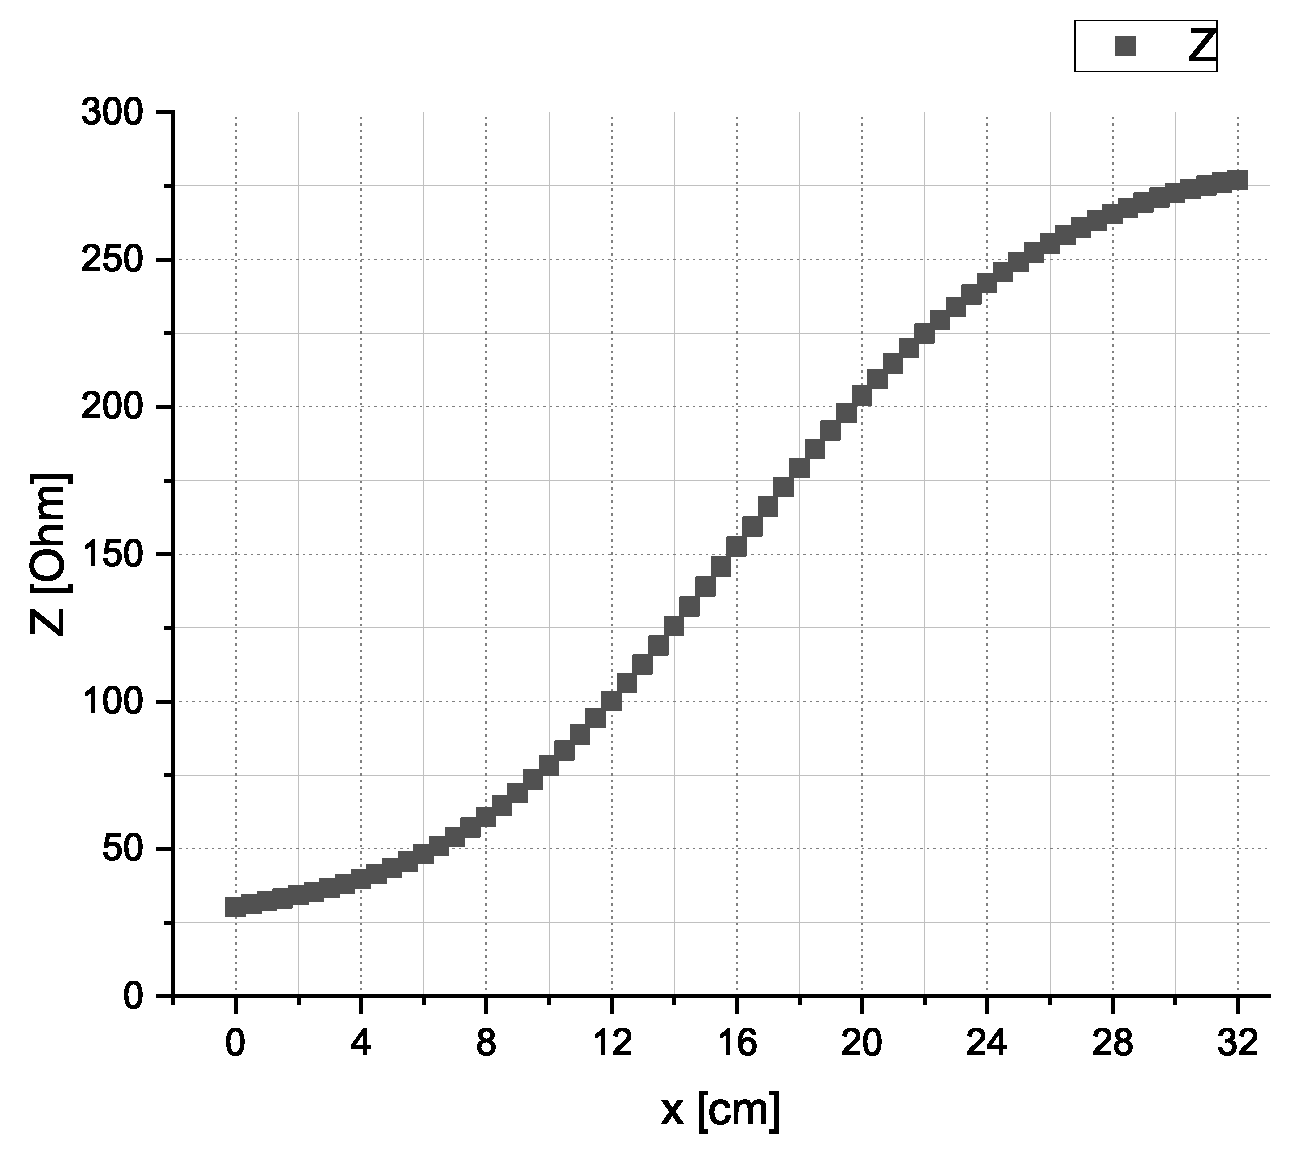
\includegraphics[scale=0.3]{Imped1}
\subcaption{Impedanz}
\label{fig:l1_imped}
\end{subfigure}%
%
\begin{subfigure}[c]{.5\textwidth}
\centering
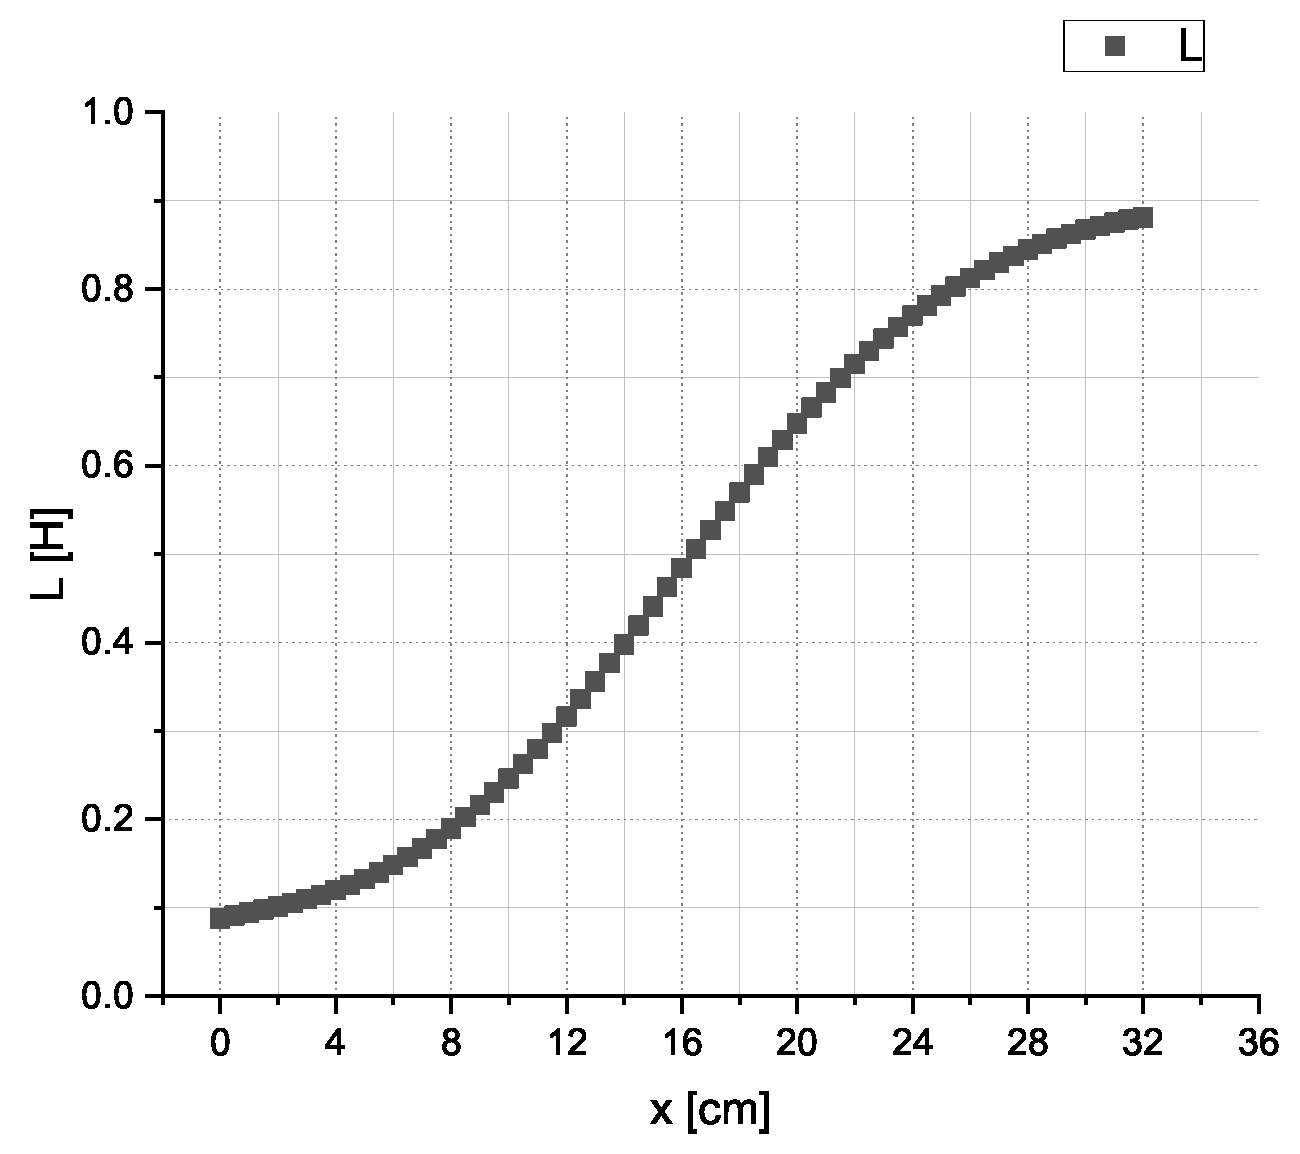
\includegraphics[scale=0.3]{Indukt1}
\subcaption{Induktivität}
\label{fig:l1_ind}
\end{subfigure}%

\caption{Messergebnisse an der Spule 1 (Massivkern)}
\label{fig:messerg_spule1}
\end{figure}

\begin{figure}[H]
\centering
\begin{subfigure}[c]{.5\textwidth}
\centering
\includegraphics[scale=0.3]{Imped2}
\subcaption{Impedanz}
\label{fig:l2_imped}
\end{subfigure}%
%
\begin{subfigure}[c]{.5\textwidth}
\centering
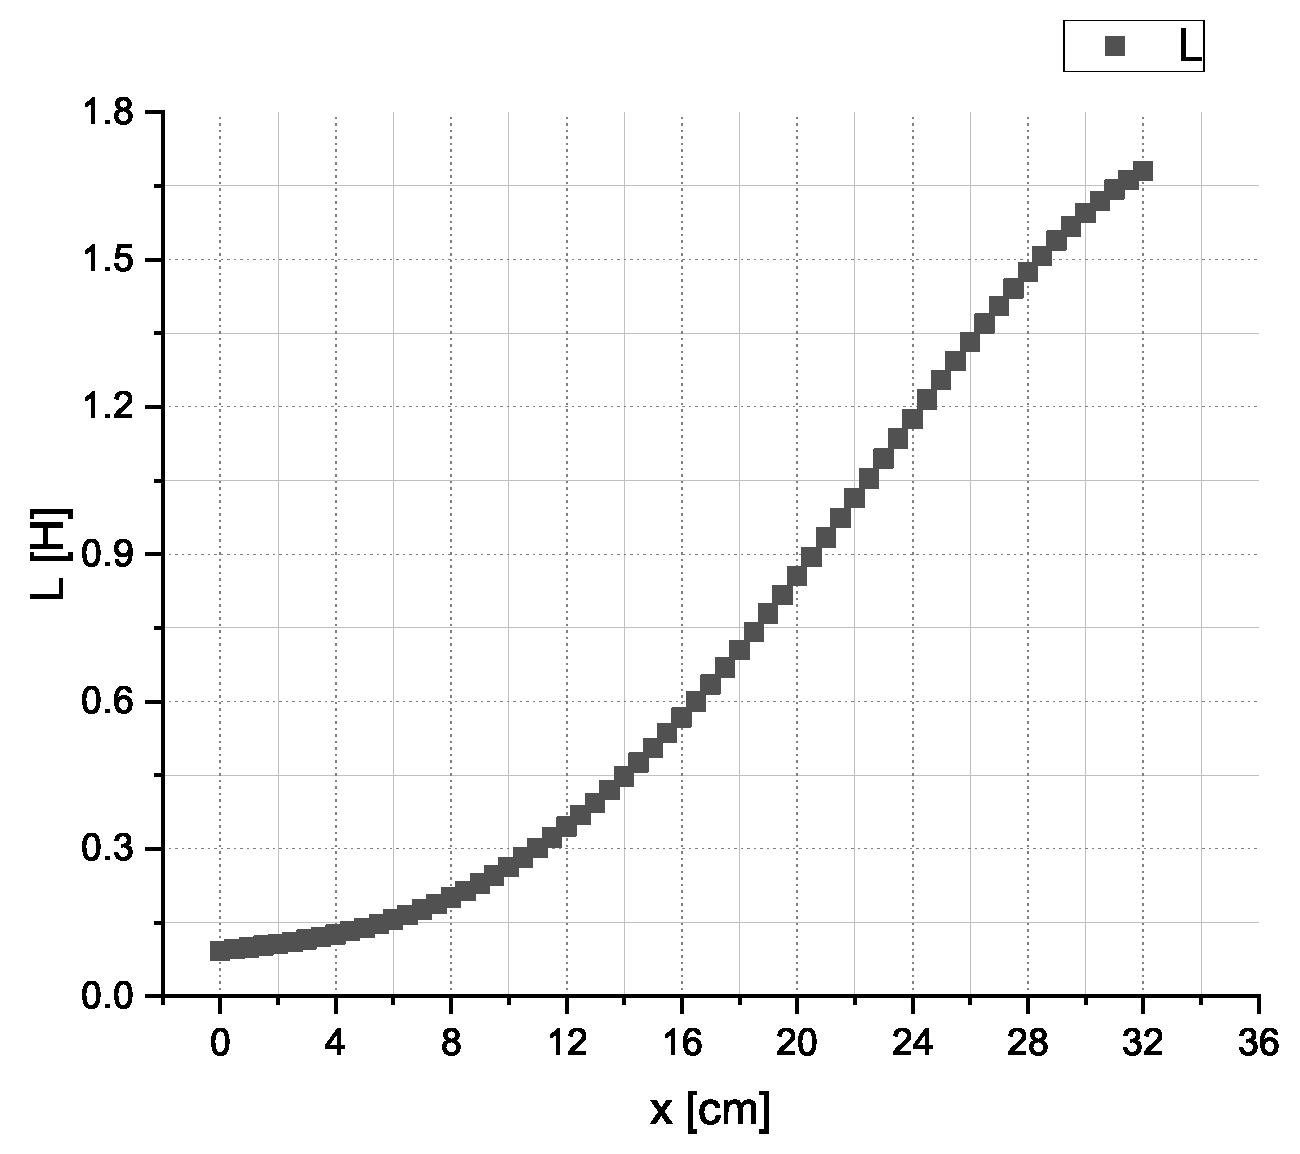
\includegraphics[scale=0.3]{Indukt2}
\subcaption{Induktivität}
\label{fig:l2_ind}
\end{subfigure}%

\caption{Messergebnisse an der Spule 2 (lammelierter Kern)}
\label{fig:messerg_spule2}
\end{figure}

\item[\textbf{Teil \rom{3}}:] \hypertarget{sec:erg_resk}{\texttt{Resonanzkreis}}

Aus Teil \rom{1} kennen wir die Kapazitäten der Kondensatoren und aus Teil \rom{2} die Induktivitäten. Wir legen fest, dass der Kern der Spule im Resonanzfall $x = 16cm$ tief eingeschoben sein soll. Aus der Tabelle \ref{fig:messerg_spule2} können wir die Induktivität der Spule ablesen; Die Frequenz im Kreis soll unterdessen $50 Hz$ betragen ($\omega = 314 \frac{1}{s}$). Damit können wir die benötigte Kapazität des Kondensators berechnen (Gleichung \ref{eq:berechn_kapa}).
\begin{equation*}
C_{reso} = \frac{1}{\omega^2 \cdot L_{16}} = \frac{1}{314^2 \frac{1}{s} \cdot 0.569 H} \approx 17.825 \mu F
\end{equation*}
Wir benötigen somit einen Kondensator mit einer Kapazität von rund $C_{res} \approx 17.825 \mu F$. Diese Kapazität können wir durch eine Verkettung von Reihen- und Parallelschaltung der Kondensatoren $C_1$ und $C_2$ erreichen (Siehe Abbildung \ref{fig:schalt_v10_konds} und \hyperlink{sec:appendix}{Appendix}).

\begin{figure}[H]
\centering
\begin{subfigure}[c]{.5\textwidth}
\centering
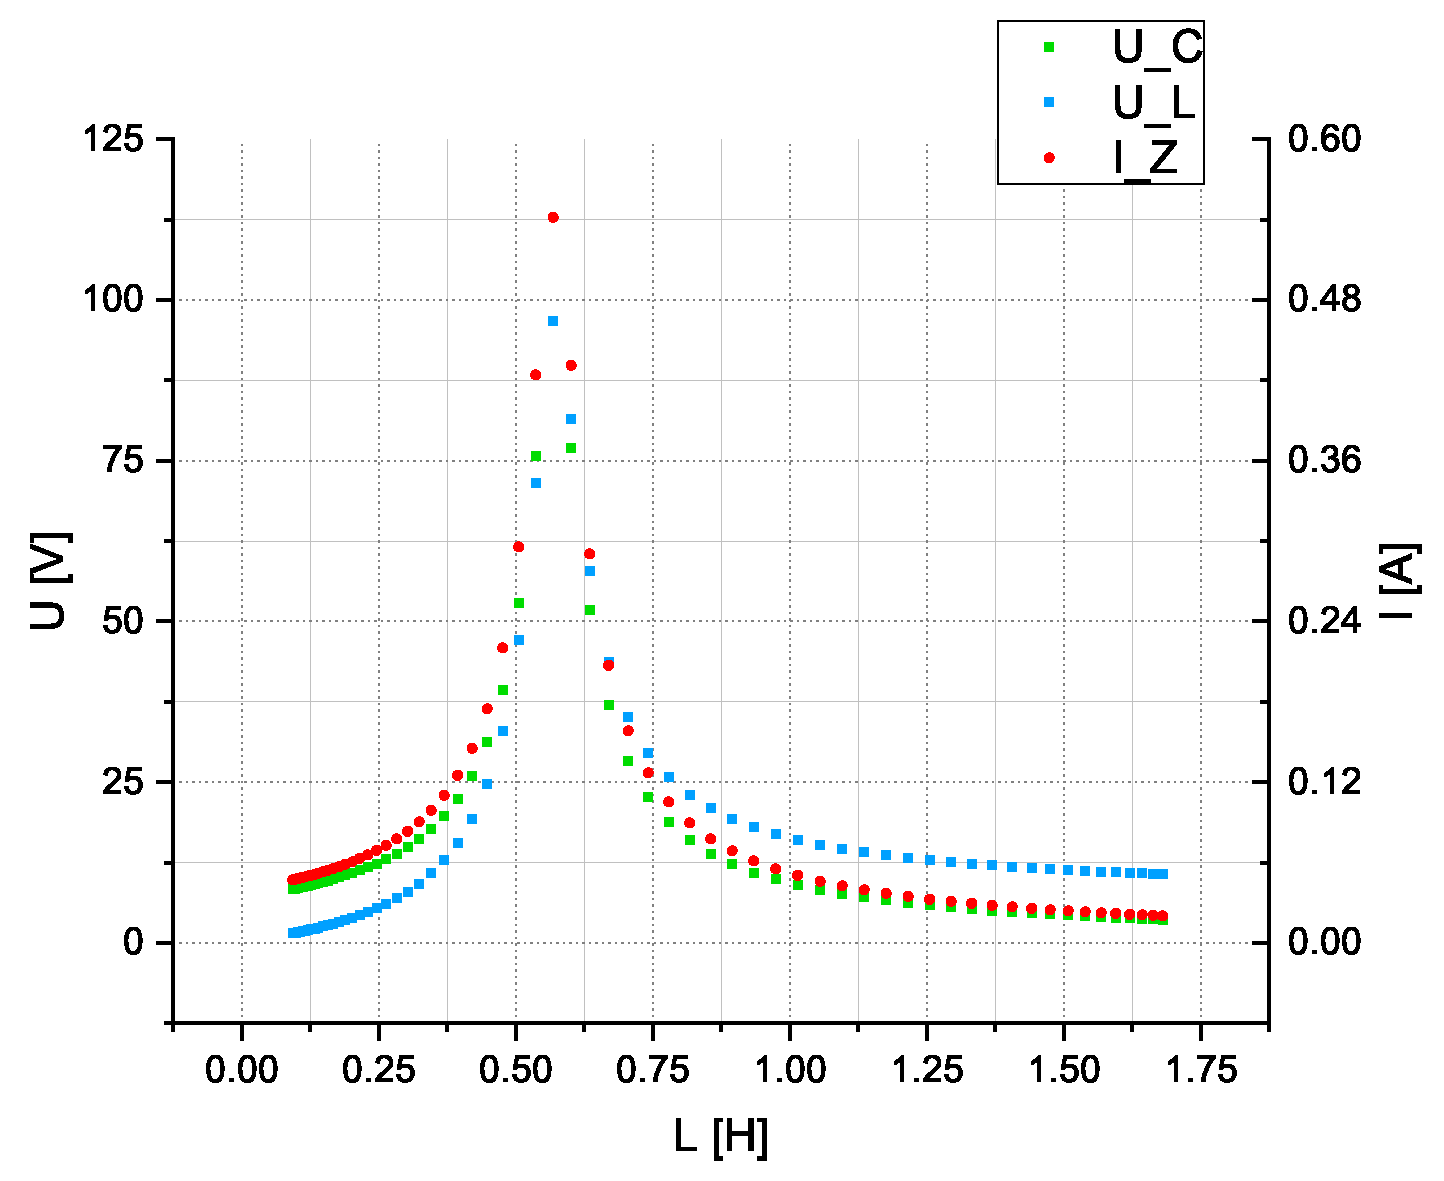
\includegraphics[scale=0.3]{Reihenschwingkreis}
\subcaption{Reihenschwingkreis.}
\label{fig:erg_res_reihe}
\end{subfigure}%
%
\begin{subfigure}[c]{.5\textwidth}
\centering
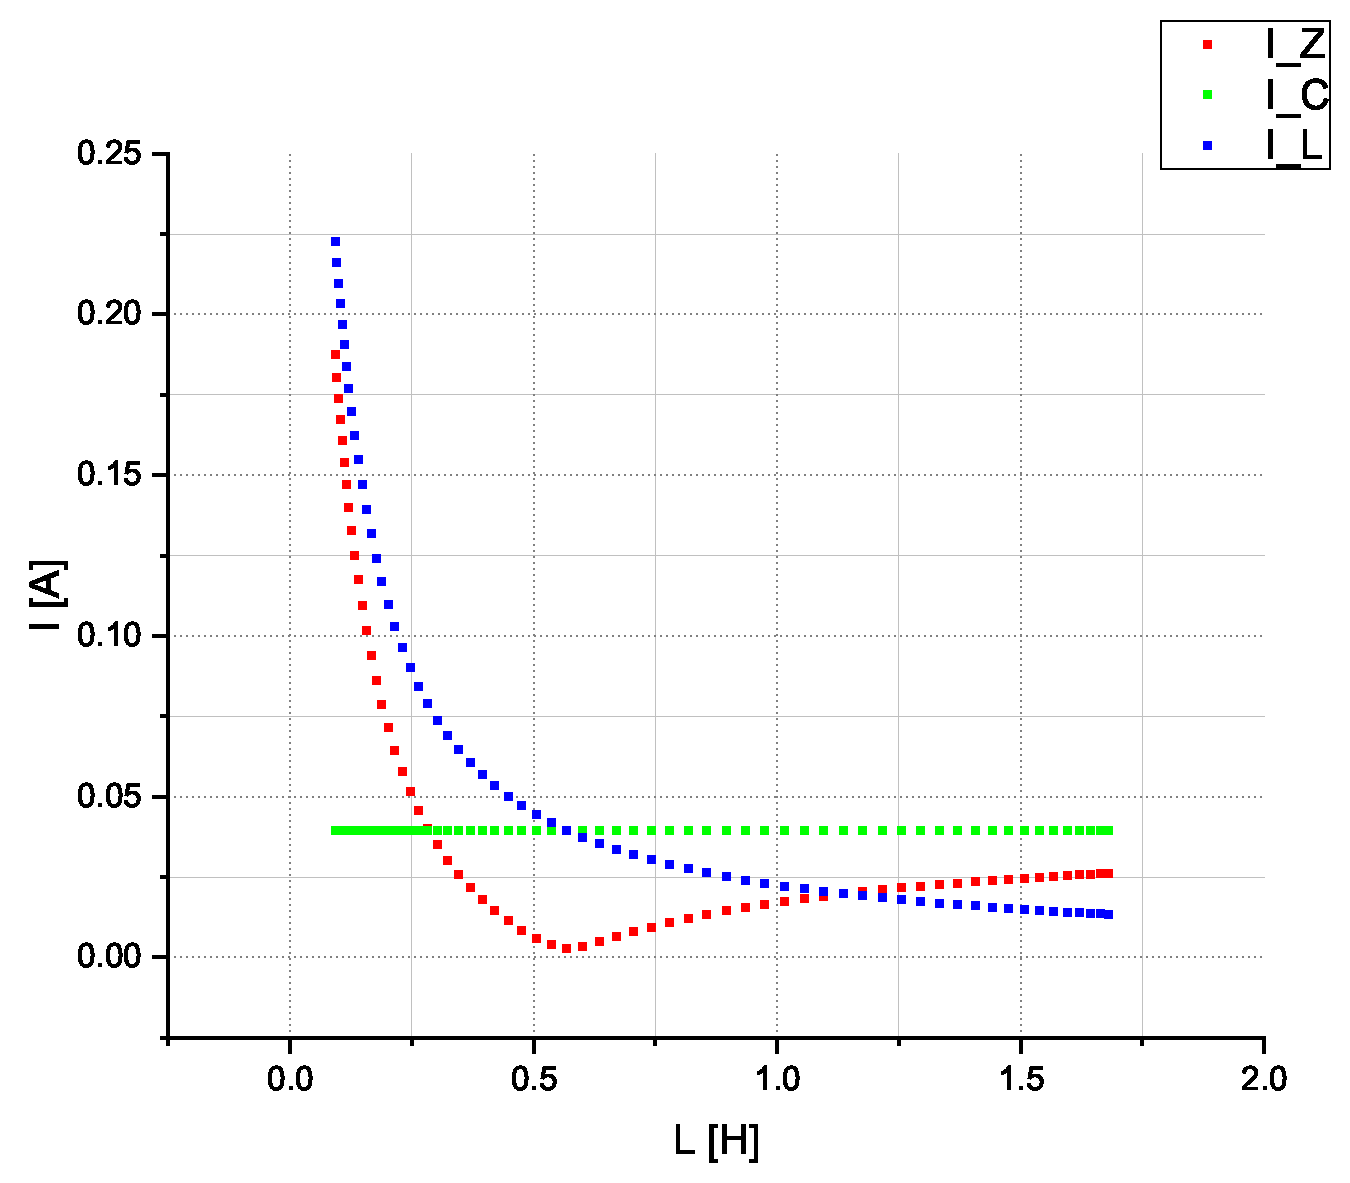
\includegraphics[scale=0.3]{Parallelschwingkreis}
\subcaption{Parallelschwingkreis.}
\label{fig:erg_res_para}
\end{subfigure}%

\caption{Messergebnisse an den Schwingkreisen.}
\label{fig:messerg_schwing}
\end{figure}
Die Graphen in Abbildung \ref{fig:messerg_schwing} zeigen die Messergebnisse an den Schwingkreisen. Dabei bezeichnet $U_C$ die Spannung am Kondensator (dem Gesamtkonstrukt), $U_L$ die Spannung an der Spule, $I_Z$ den Strom in der Zuleitung bzw. im Schwingkreis (an der Spannungsquelle gemessen), $I_C$ den Strom am Kondensator (bzw. -Konstrukt) und $I_L$ den Strom an der Spule.
\end{itemize}
\end{flushleft}

\subsection{Diskussion der Messergebnisse}
\begin{flushleft}
\begin{itemize}
\item[\textbf{Teil \rom{1}}:] Wir haben die Kapazitäten bestimmt. Der Kondensator $C_1$ besitzt eine Kapazität von rund $102.4 \mu F$ und eine Impedanz von rund $31.1 \Omega$; Die Werte für Kondensator $C_2$ sind $15.28 \mu F$ und $208.37 \Omega$.

Bei der Parallelschaltung summieren sich die beiden Kapazitäten - die Gesamtkapazität vergrößert sich -, bei der Reihenschaltung verkleinert sich die Kapazität. Für die Impedanz verhält es sich genau anders herum: bei der Reihenschaltung vergrößert sich die Impedanz durch die Addition beider Impedanzen, während sich die Impedanz der Parallelschaltung verkleinert.

Wir wollen nun noch überprüfen, ob die angegebenen Zusammenhänge bei Kondensatoren in Parallel- und Reihenschaltung bezüglich der Kapazität (Gleichungen \ref{eq:kond_para} und \ref{eq:kond_reihe}) korrekt sind. Dazu berechnen wir die jeweilige Gesamtkapazität mit den gemessenen Werten für die Kondensatoren $C_1$ und $C_2$.

\begin{align*}
C_{\parallel} &= \sum_i C_i & \frac{1}{C_{\mid}} &= \sum_i \frac{1}{C_i} \\
C_{\parallel} &= C_1 + C_2 & \frac{1}{C_{\mid}} &= \frac{1}{C_1} + \frac{1}{C_2} \\
C_{\parallel} &= 102.395 \mu F + 15.284 \mu F & \frac{1}{C_{\mid}} &= \frac{1}{102.395 \mu F} + \frac{1}{15.284 \mu F} \\
C_{\parallel} &= 117.679 \mu F & C_{\mid} &\approx 13.299 \mu F
\end{align*}
Die berechneten Werte stimmen mit den Messwerten aus Tabelle \ref{tab_messerg_kond} genau überein.

\item[\textbf{Teil \rom{2}}:] Die Messergebnisse zeigen, dass bei beiden Spulen sowohl Impedanz, als auch Induktivität mit der Einschubtiefe steigen (Abbildungen \ref{fig:messerg_spule1} und \ref{fig:messerg_spule2}). Hierbei ist zu erkennen, dass das beide Größen an beiden \glqq Enden\grqq\hspace{1pt} asymptotisch laufen, also nicht gradlinig.

Beide Spulen besitzen dabei eine \glqq eisenfreie Induktivität\grqq\hspace{1pt} von rund $L_{0} = 0.09 H$. Bei der Spule $L_1$ mit dem \textit{Massivkern} (Tabelle \ref{tab:messerg_spul1}, Abbildung \ref{fig:messerg_spule1}) steigen Impedanz und Induktivität dabei auf weniger große Werte als bei Spule $L_2$ (Tabelle \ref{tab:messerg_spul2}, Abbildung \ref{fig:messerg_spule2}). Für $x = 32$ sind die Werte für Spule zwei fast doppelt so groß, wie für Spule eins.

\begin{figure}[H]
\centering
\includegraphics[scale=0.3]{Phasen_Spulen_Spice}
\caption{Phasen zischen Spulenstrom beider Spulen und Gesamtspannung.}
\label{fig:phasen_spulen_0_32}
\end{figure}

Die Abbildung \ref{fig:phasen_spulen_0_32} zeigt die Phasenverschiebung zwischen der Gesamtspannung und dem Strom an den Spulen für $x = 0cm$ und $x = 32cm$. Dabei sind die \textcolor{green}{grünen Linien} die Werte für \textcolor{green}{Spule 1} (Massivkern) \textcolor{blue}{blauen Linien} zu \textcolor{blue}{Spule 2}. Die flachen Kurven sind zu $x = 32 cm$, die hohen zu $x = 0 cm$. Die \textcolor{red}{rote Kurve} zeigt die \textcolor{red}{Gesamtspannung}.

Wir können in der Graphik sehen, dass sich die Phasenverschiebung zwischen Strom und Spannung deutlich ändert, wenn die Kerne eingeschoben werden. Für $x = 0$ liegt die Verschiebung für beide Spulen bei rund $\Delta t = 3.5 ms$ - umgerechnet eine Phasenverschiebung von $\varphi = (3.5 \div 10) \pi (rad) = 63^{\circ} (grad)$. Für den Massivkern ändert sich die Phasenverschiebung zu $\varphi = (0.2 \div 10) \pi (rad) = 18^{\circ} (grad)$ ($\Delta t = 2 ms$); für den lamellierten Kern ändert es sich zu $\varphi = (5 \div 10) \pi (rad) = 90^{\circ} (grad)$ ($\Delta t = 5 ms$).

\item[\textbf{Teil \rom{3}}:] Die Messergebnisse (Abbildung \ref{fig:messerg_schwing}) zeigen eine klare Differenz des Verhaltens zwischen Reihen- und Parallelschwingkreis. Beim Reihenschwingkreis ist zu erkennen, dass sowohl Spannung als auch Strom bei etwa $L \approx 0.57$ ein \textbf{Maximum} besitzen. Aus Tabelle \ref{tab:messerg_spul2} können wir ablesen, dass diese Induktivität bei $x = 16cm$ auftritt. Dieses Maximum stellt also unser Resonanzfall dar.

Beim Parallelschwingkreis ist in diesem Fall der Strom im Schwingkreis $I_Z$ an einem \textbf{Minimum}. Der Strom an der Spule ist derweil identisch zu den Werten aus der Messung von Teil \rom{2} (Tabelle \ref{tab:messerg_spul2}) und der Strom am Kondensator ist durchgehend konstant.

Die Messungen zeigen, dass in einem Parallelschwingkreis Spule und Kondensator quasi wie abgekopllet voneinander sind und keine Wirkungen aufeinander zeigen. Im REihenschwingkreis hingegen funktioniert wie in der \hyperlink{theo-res}{Theorie} beschrieben.
\end{itemize}
\end{flushleft}

\section{Fazit}
\begin{flushleft}
Der Versuch 9 und der Versuch 10 zeigen das Verhalten von Kondensator und Spule im Wechselstromkreis und das Zusammenspiel beider Komponenten.
%\begin{itemize}
%\item[\textbf{Teil \rom{1}}:] 
%
%\item[\textbf{Teil \rom{2}}:] 
%
%\item[\textbf{Teil \rom{3}}:] 
%\end{itemize}
\end{flushleft}

\begingroup
\raggedright
\sloppy
\printbibliography[heading=bibintoc,title={6 \hspace{6pt} Literatur}]
\endgroup

\newpage

\section*{Appendix}
\begin{flushleft}
\hypertarget{sec:appendix}{Anbei} liefere ich meine für dieses Protokoll geschriebenen Pythonscripte mit, die ich für die Bearbeitung des Versuches verwendet habe.
\end{flushleft}

\paragraph{Datenauswertung}
\begin{flushleft}
Anbei mein script zum Auswerten der Daten aus den \textbf{LTSpice} \texttt{.log}-Dateien. Es dient zum Extrahieren der \texttt{.meas}-Daten zum einfachen Importieren in \texttt{Origin Pro}. Die Skripte sind für die Verwendung mit \texttt{IDLE} optimiert.

\scriptsize
\begin{minted}[xleftmargin=10pt,linenos]{python}
"""Small script to extract the LTSpice Data (logs) for usage with Origin Pro"""

def main(case: int = 0):
    """Main method

    @param case: case = 1 => add steps for core (x) in output
    """

    # Input files
    inp_files = ["Reihenschwing", "Parallelschwing"]

    for file in inp_files:
        input_file = open(file+".log","r")
        lines = input_file.readlines()

        # Needed variables for extraction
        transformed = []
        data = []
        index = -1
        meas = False

        # First two hits have to be excluded
        curr_step = -1

        # Total number of lines with data
        max_steps = 65

        if (case == 1):
            data.append([])
            for i in range(1,max_steps+1):
                step_x = (i-1)/2
                step_x = str(step_x).replace(".",",")
                data[0].append(step_x)

                index += 1

        for line in lines:
            # Indicator where the extraction should start
            if line.__contains__("Measurement"):
                meas = True
                data.append([])
                index += 1
                curr_step = -1
            elif (curr_step == max_steps+1):
                meas = False

            if (meas):
                if curr_step > 0:
                    # Extract the .meas data
                    # Attention: Origin uses the format 1.000,00 for imports
                    # (or my settings are incorrect)
                    dat = line.split('\t')[1].replace(".",",")

                    # Calculate the x (depth of core)
                    data[index].append(dat)

                curr_step += 1

        # Reformat data list
        # data = [[1, 2, 3, 4, ...], [a, b, c, d, ...]]
        # output = [[1, a], [2, b], [3, c], ...]
        output = []
        for jj in range(len(data[0])):
            rearrange = ""
            for ii in range(len(data)):
                # Tab seperated
                rearrange += data[ii][jj] + "\t"
            output.append(rearrange[:-1]+"\n")
        print(output)

        # Write data to file        
        with open(file+"_extracted.dat", "w+") as output_file:
            output_file.writelines(output)
        


if __name__ == "__main__":
    main()
\end{minted}
\normalsize
\end{flushleft}

\paragraph{Kapazitätenrechnung}
\begin{flushleft}
Das folgende script dient zum Rechnen mit Kapazitäten. Ich habe es geschrieben, um einfacher mit den Kapazitäten zu rechnen und um eine Kombination der Kapazitäten für Versuch 10 (Teil \rom{3}) zu ermitteln. Die \textit{main} Methode beinhaltet die in Versuch 9 ermittelten Kapazitäten sowie die Berechnungen für die Kapazität $C_{res}$ aus diesen.

\scriptsize
\begin{minted}[xleftmargin=10pt,linenos]{python}
"""Small program for calculations with capacitys of condensators"""

class Cond():
    """Class for Condensators"""

    def __init__(self, c):
        """Constructor"""
        self.c =  c

    def reihe(self, caps: list):
        """Reiehnschaltung"""

        values = [1 / caps[i].c for i in range(len(caps))]
        values.append(1 / self.c)
        return 1 / sum(values)

    def para(self, caps: list):
        """Parallelschaltung"""

        values = [caps[i].c for i in range(len(caps))]
        values.append(self.c)
        return sum(values)


def main():
    """Initialise some capacitys"""

    global c1, c2, cpa, creih, cl, cr_p, cr, cges

    c1 = Cond(102.395*10**(-6))
    c2 = Cond(15.284*10**(-6))
    cpa = Cond(c1.para([c2]))
    creih = Cond(c1.reihe([c2]))

    cl = Cond(c2.reihe([c1, c2]))
    cr_p = Cond(c1.para([c2]))
    cr = Cond(c1.reihe([cr_p, c1, c2]))
    cges = Cond(cl.para([cr]))


if __name__ == "__main__":
    main()
\end{minted}
\normalsize

\end{flushleft}

\end{document}
